\documentclass[notes]{beamer}
\usetheme{Rochester}

\usepackage{graphicx}
\usepackage{amsmath,amssymb}
\usepackage{ gensymb }

\title{Advanced Projects in Exoplanets}
\subtitle{The RM Effect}
\author{Dina Sofia Mortensen \& Jesper Dam Knudgaard}
\institute{Stellar Astrophysics Centre, Aarhus University}
\date{\today}

\begin{document}

\begin{frame}
\titlepage
\end{frame}

\section{The RM Effect}

\begin{frame}
\frametitle{Transiting Exoplanets}
	\begin{figure}
		\centering
		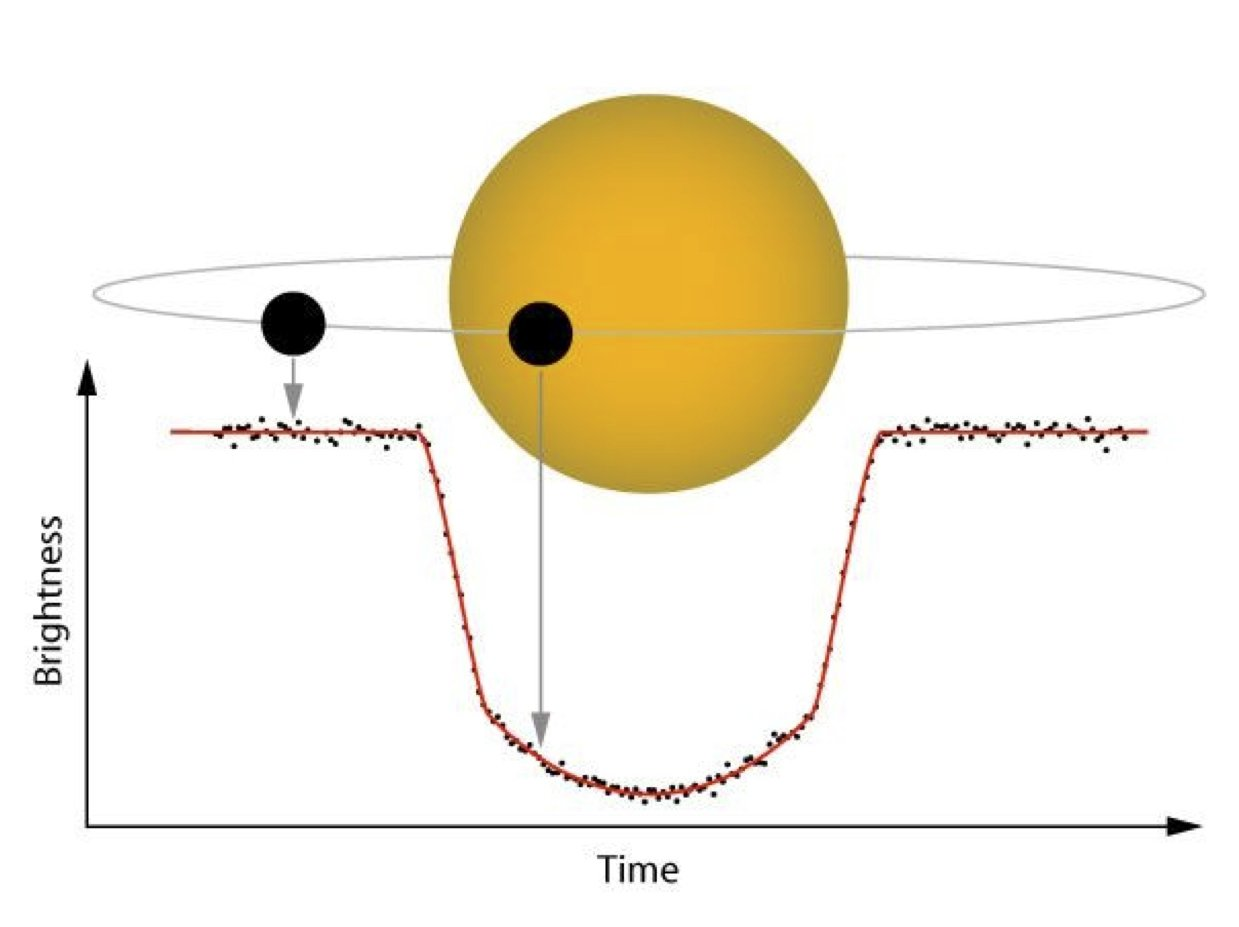
\includegraphics[width = 0.7\columnwidth]{Transit.jpg}
		\caption{\textit{Credit ESO}}
		\label{fig:transit} 
	\end{figure}
\end{frame}

\begin{frame}
\frametitle{Rossiter-McLaughlin}
	\begin{figure}
		\centering
		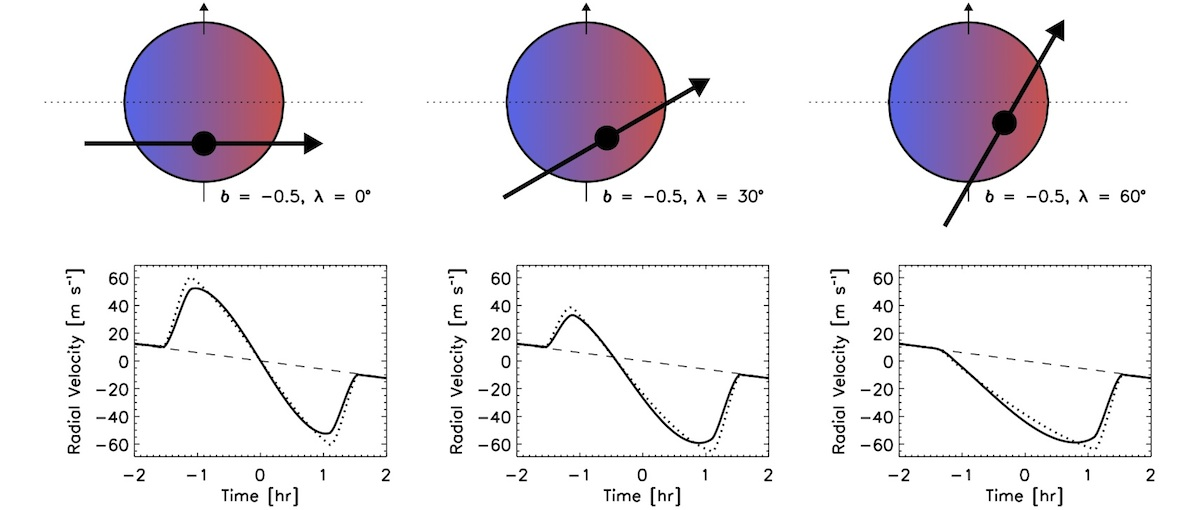
\includegraphics[width=\textwidth]{winnwhites.jpg}
		\caption{\url{https://wasp-planets.net/tag/rossiter-mclaughlin-effect/}}
		\label{fig:rm_effect}
	\end{figure}
\end{frame}



\end{document}
